\chapter[Lecture 2]{}\label{lec2}

\section*{Crystal Structure}

How much two atoms can come cluse?

Lennard-Zones potential (1924)
\begin{figure}[H]
\centering
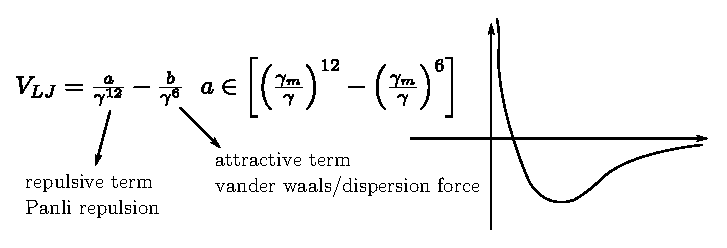
\includegraphics[scale=.9]{images/lecture2/fig1.eps}
\end{figure}

Buckingham potential/Richard potential
$$
V_{B}=r\left[l^{-r/r_{0}}-\left(\dfrac{r_{0}}{r}\right)^{6}\right]
$$
Liquid Crystals - A state of matter possessing properties of conventional liquids and solids.
\begin{center}
\begin{tabular}{>{\raggedright}p{4.5cm}>{\raggedright}p{4.5cm}p{4.5cm}<{\raggedright}}
\multicolumn{1}{c}{\bf Thermotropic} & \multicolumn{1}{c}{\bf Lyotropic} & \multicolumn{1}{c}{\bf Metallotropic}\\[3pt]
Phase transition as a function of temperature & Phase transition as a function of temperature and density & Phase transition depends on temperature density and ration of organic, inorganic molecules\\[6pt]
Organic & Organic & Both organic and inorganic
\end{tabular}
\end{center}
\begin{description}
\item[Nematic :] liquid like but has long range directional order.

\item[Smectic :] liquid within the layer.

\item[Chiral :]
\end{description}

\section*{Crystal Structure}

\begin{description}
\item[BASIS :] An ideal crystal is constructed by the infinite repetition of identical groups of atoms. A group is called {\bf basis}.

\item[Lattice :] The set of mathematical points to which the basis is attached is called the {\bf lattice}.

\item[Translation Vectors :] If $a_{1}$, $a_{2}$ and $a_{3}$ are three translation vectors in three dimensions defines the lattice so that the arrangement of atoms looks the same at $r$ as it is at $r'$. Then,
$$
\fbox{$r'=r+\sum\limits^{3}_{i=1}n_{i}a_{i}$}\quad n_{i}\to i=1,2,3\quad\text{are integers.}
$$

\item[Primitive Lattice :] If any two equivalent points in a lattice can be connected by the three translation vectors the lattice is called {\bf Primitive Lattice}.

\item[Primitive Vectors :] The smallest possible translation vectors that form the primitive lattice is called {\bf Primitive Vectors}.

The volume $a_{1},a_{2}\times a_{3}$ is the smallest volume that can serve as building block of the crystal structure.

\item[Crystal axes :] Primitive translation vectors are defined as {\bf Crystal axes}. 

Sometimes non-primitive vectors are used to define crystal axes if they have some simple relation to the crystal symmetry.

\item[Bravais Lattice :] An infinite array of lattice points with an arrangement and orientation that appears exactly the same from whichever point the array is viewed.

If $\overrightarrow{R}$ is the position vector of a Bravais lattice, then it can be defined as $\overrightarrow{R}=\sum\limits_{i=1}n_{i}\overrightarrow{a}_{i}$.

\item[Basis :] Basis may consists of one or more points. In the case of more than one point $\to$ the constituent points can be defined as
$$
r_{j}=\sum\limits_{i-1}x_{ij}a_{i}\quad 0\leq x_{ij}\leq 1
$$
\end{description}

\section*{Two Dimension}
\begin{figure}[H]
\centering
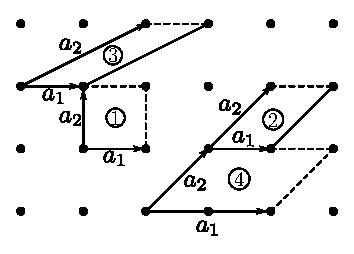
\includegraphics{images/lecture2/fig2.eps}
\end{figure}
Case (1), (2) and (3) are all primitive vectors. They all have same volume.

\smallskip

\noindent
Case (4) is not a primitive vector, they cannot form the whole lattice. Volume = $2\times{}$ primitive cell.
\begin{description}
\item[Primitive Lattice Cell :] Minimum Volume Cell, that can fill up the whole lattice space via suitable crystal translation operations.
\end{description}

For an elemental lattice, there is one lattice point per primitive cell.

Cube $\to$ each corner contribute $\dfrac{1}{8}$th, eight corners.

Total Contribution = $\dfrac{1}{8}\times 8=1$

$V_{c}=|a_{1},a_{2}\times a_{3}|$

Basis associated is a primitive cell is called primitive basis.

No basis contains fewer atoms than a primitive basis.
\begin{description}
\item[Wigner-Seitz Cell :] Draw perpendicular bisectors of each of the lines connecting the nearest neighbors. The volume enclosed is called {\bf Wigner-Seitz Cell.}
\end{description}

\section*{Fundamental Types of Lattices}

A single molecule can have any degree of rotation symmetry. But crystal cannot have $\to$
\begin{center}
\begin{tabular}{lccccc}
Allowed rotations $\to$ & $2\pi$, & $2\pi/2$, & $2\pi/3$, & $2\pi/4$, & $2\pi/6$\\[3pt]
Degree & 1 & 2 & 3 & 4 & 6
\end{tabular}
\end{center}

Five and Seven - fold rotation cannot fill up the whole space. e.g. For five fold rotational symmetry $\to$ $\theta=2\pi/5$ around the centre of rotation.
\begin{figure}[H]
\centering
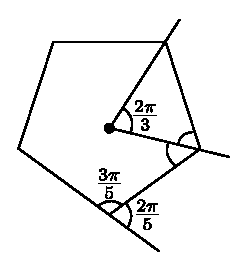
\includegraphics{images/lecture2/fig3.eps}
\end{figure}

$\therefore \ \dfrac{2\pi}{3\pi/5}=\dfrac{10}{3}$ Not an integer.

\smallskip

$\therefore$ \ Five fold rotational symmetry cannot fill up the space.

\smallskip

{\bf $\to$ Qusicrystals.}

\smallskip

Possess perfect long-range order but no translational symmetry.

In two dimension:
\begin{itemize}
\item[(i)] Octagonal $\to$ 8-fold symmetry (Primitive and body centered lattices)

\item[(ii)] Decagonal $\to$ 10-fold symmetry (Primitive)

\item[(iii)] Dodecagonal $\to$ 12-fold symmetry (Primitive)
\end{itemize}

In three dimension $\to$

Icosahedral Quasicrystal

($12\times 5$-fold; $20\pi 3$-fold; $30\times 2$-fold)

(Primitive, body-centered and face centered)

\section*{Penrose filing}

Aperiodic filing to fill up two dimensional space:
\begin{itemize}
\item[P1 :] Uses pentagon, five pointed star (a pentagram), a boat ($3/5$th of a star); diamond (thin rhombus)

\item[P2 :] Kite and dart
\begin{figure}[H]
\centering
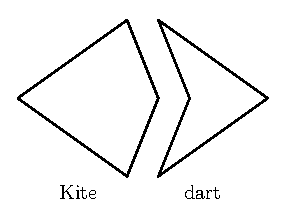
\includegraphics{images/lecture2/fig4.eps}
\end{figure}

\item[P3 :] Rhombus pair
\begin{figure}[H]
\centering
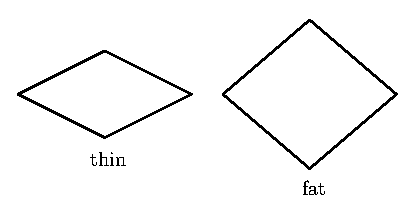
\includegraphics{images/lecture2/fig5.eps}
\end{figure}
\end{itemize}

\section*{Two Dimensional lattice}
\begin{figure}[H]
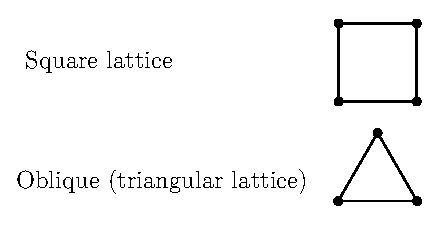
\includegraphics{images/lecture2/fig6.eps}

\medskip

\noindent
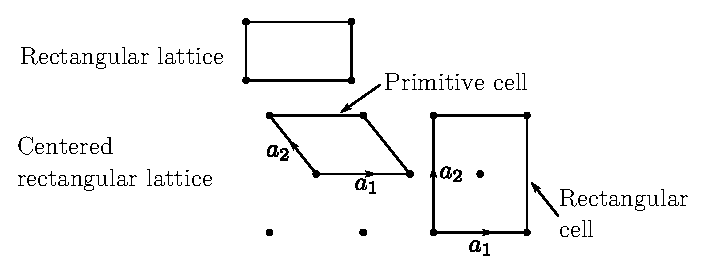
\includegraphics{images/lecture2/fig7.eps}
\end{figure}
All are Bravais lattice

\subsection*{Graphene}
\begin{figure}[H]
\centering
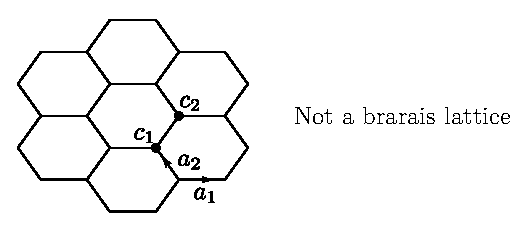
\includegraphics{images/lecture2/fig8.eps}
\end{figure}

Basis contains two non-equivalent carbon atoms $\left[\begin{smallmatrix} C_{1}\\ C_{2}\end{smallmatrix}\right]$ $\to$ lattice translation vectors $\overline{a}_{1}$, $\overline{a}_{2}$.



